% Artigo final do POC I — modelo IEEE (IEEEtran, conferência).
% Compilar: pdflatex artigo && bibtex artigo && pdflatex artigo && pdflatex artigo
% (ou latexmk -pdf artigo). Figuras: scripts/paper_figs.py; tabelas: scripts/paper_tables.py.
\documentclass[conference,a4paper]{IEEEtran}

\usepackage[utf8]{inputenc}
\usepackage[T1]{fontenc}
\usepackage[brazil]{babel}
\usepackage{amsmath,amssymb}
\usepackage{icomma}
\usepackage{graphicx}
\usepackage{booktabs}
\usepackage{longtable}
\usepackage{array}
\usepackage{cite}
\usepackage{url}
\usepackage[hidelinks]{hyperref}

\graphicspath{{figs/}}
\newtheorem{lema}{Lema}
\newtheorem{proposicao}{Proposição}
\renewcommand{\IEEEkeywordsname}{Palavras-chave}
\newcommand{\tabela}[1]{\input{tabelas/#1}}

\begin{document}

\title{Aprendizado de Máquina para Escolhas Gulosas\\em Coloração de Grafos: Base de Dados,\\Análise Exploratória e Prova de Conceito}

\author{\IEEEauthorblockN{Lucas Affonso Pires}
\IEEEauthorblockA{Departamento de Ciência da Computação\\
Universidade Federal de Minas Gerais\\
Belo Horizonte, Brasil}
\and
\IEEEauthorblockN{Marcio Costa Santos (orientador)}
\IEEEauthorblockA{Departamento de Ciência da Computação\\
Universidade Federal de Minas Gerais\\
Belo Horizonte, Brasil}}

\maketitle

\begin{abstract}
Algoritmos gulosos de coloração de vértices colorem um vértice por vez com a menor cor
permitida, e o número de cores obtido depende da regra que escolhe o próximo vértice. Este
trabalho, primeira etapa de um projeto de dois semestres, investiga se um modelo de
aprendizado de máquina pode aprender essa escolha passo a passo. Implementamos as heurísticas
ordem aleatória, Welsh-Powell, DSATUR e RLF como regras de escolha sobre um mesmo estado
parcial e construímos uma base reprodutível com 2.818 grafos Erdős–Rényi e Barabási–Albert,
7,3 milhões de passos registrados e 858.790 candidatos rotulados por \emph{rollout}. Provamos
que a coloração ``oráculo'' induzida pelos rótulos nunca usa mais cores que a melhor entre
DSATUR e RLF; ela usa menos em 55\% dos grafos rotulados. A análise exploratória mostra que a
disputa se dá apenas entre RLF e DSATUR e que a família do grafo praticamente determina a
vencedora. Na prova de conceito, um classificador por \emph{gradient boosting} acerta 97,2\% das
escolhas nos passos decisivos de validação, contra 89,3\% da sugestão do RLF; de ponta a ponta,
porém, a política aprendida empata com a melhor heurística em 96\% dos grafos, pois aprende a
seguir o RLF ou o DSATUR conforme a família, e seus poucos erros por passo se acumulam. No teste
final com 127 instâncias DIMACS, usado uma única vez, a política empata com a melhor heurística
em 90\% das instâncias, usa menos cores em uma e mais em 9\%, enquanto o oráculo supera a
melhor heurística em 24\% das instâncias com até 500 vértices. As melhorias do modelo ficam
para o segundo semestre (POC~II).
\end{abstract}

{\renewcommand{\abstractname}{Abstract}
\begin{abstract}
Greedy vertex-colouring algorithms colour one vertex at a time with the smallest available
colour, and the number of colours depends on the rule that picks the next vertex. We study
whether a machine-learning model can learn this choice step by step. We implement random
order, Welsh-Powell, DSATUR and RLF as choice rules over a common partial state and build a
reproducible dataset of 2,818 Erdős–Rényi and Barabási–Albert graphs with 858,790
rollout-labelled candidates; the induced oracle colouring provably never uses more colours
than the best of DSATUR and RLF and uses fewer in 55\% of the labelled graphs. A gradient
boosting classifier picks an optimal candidate in 97.2\% of the decisive validation steps
(RLF's suggestion: 89.3\%), but end to end it ties the best heuristic in 96\% of the graphs: it
learns to follow RLF or DSATUR depending on the graph family, and its few per-step errors
accumulate. In the single final test on 127 DIMACS instances, the policy ties the best
heuristic on 90\% of them, improving on one and losing on 9\%, whereas the oracle beats the
best heuristic on 24\% of the instances with up to 500 vertices. Model improvements are left
to the second semester of the project.
\end{abstract}}

\begin{IEEEkeywords}
coloração de grafos, algoritmos gulosos, aprendizado de máquina, \emph{rollout}, seleção de
algoritmos.
\end{IEEEkeywords}

% =====================================================================================
\section{Introdução}\label{sec:intro}

Colorir os vértices de um grafo $G=(V,E)$ é atribuir a cada vértice uma cor de modo que
vértices adjacentes recebam cores diferentes, usando o menor número possível de cores, o
número cromático $\chi(G)$. Decidir se $G$ admite uma coloração com $k \ge 3$ cores é
NP-completo~\cite{karp1972,garey1979}, de modo que métodos exatos só são práticos em
instâncias pequenas ou com estrutura especial. O problema modela alocação de registradores
em compiladores, atribuição de frequências, montagem de horários e escalonamento com
conflitos~\cite{lewis2021,malaguti2010}.

Na prática, usam-se algoritmos gulosos: os vértices são coloridos um por vez, cada um com a
menor cor ainda não usada por seus vizinhos. O resultado depende da \emph{regra de escolha}
do próximo vértice. As regras clássicas, como a ordem por grau decrescente de Welsh e
Powell~\cite{welsh1967}, a saturação máxima do DSATUR~\cite{brelaz1979} e a construção por
conjuntos independentes do RLF~\cite{leighton1979}, não se dominam: o desempenho relativo muda
com a densidade e a estrutura do grafo~\cite{lewis2021}. Isso sugere que a melhor escolha em
cada passo depende de características locais da instância, o que aproxima o problema da
seleção de algoritmos~\cite{rice1976,musliu2013} e do aprendizado de heurísticas
construtivas~\cite{khalil2017,bengio2021}.

O \textbf{objetivo geral} do projeto, a ser concluído no segundo semestre (POC~II), é
desenvolver e avaliar um modelo que, a cada passo da construção gulosa, escolha o próximo
vértice de modo a usar número de cores igual ou menor que as heurísticas clássicas. Os
\textbf{objetivos do POC~I}, tratados neste texto, foram: (i)~revisar a literatura;
(ii)~implementar as heurísticas de referência; (iii)~construir uma base de dados de grafos
sintéticos e de \emph{benchmark}; (iv)~executar as heurísticas registrando atributos de cada
passo e o número de cores; (v)~fazer uma análise exploratória; (vi)~implementar uma prova de
conceito do modelo preditivo; e (vii)~consolidar base, código e resultados.

As \textbf{contribuições} são: (a)~um arcabouço em que toda heurística é uma regra de escolha
sobre o mesmo estado parcial, com três implementações equivalentes do RLF, o que permite
misturar regras ao longo de uma construção (Seção~\ref{sec:heur}); (b)~uma base de dados em
camadas, reprodutível, com rótulos por passo obtidos por \emph{rollout} com duas
políticas-base e garantia de melhoria (Seções~\ref{sec:base} e~\ref{sec:rotulos}); (c)~uma
análise exploratória que identifica o que distingue as heurísticas e quantos passos de fato
exigem decisão (Seção~\ref{sec:res-eda}); (d)~uma prova de conceito avaliada não só por
acurácia por passo, mas de ponta a ponta, em grafos nunca vistos e num teste único com 127
instâncias DIMACS (Seções~\ref{sec:res-modelo} e~\ref{sec:res-dimacs}); e (e)~código
documentado, com 43 testes automatizados, que regenera todos os resultados
(Apêndice~\ref{ap:repro}).

O resultado central é um alerta metodológico: um classificador com 97\% de acerto por passo
produz colorações apenas iguais às da melhor heurística. As melhorias do modelo que atacam
essa limitação foram planejadas, mas \textbf{ficam para o POC~II} (Seção~\ref{sec:conclusao}).

O texto está organizado assim: a Seção~\ref{sec:ref} apresenta o referencial teórico e os
trabalhos correlatos; a Seção~\ref{sec:dev} descreve o desenvolvimento; a
Seção~\ref{sec:res} apresenta e discute os resultados; e a Seção~\ref{sec:conclusao} conclui e
apresenta os trabalhos futuros. Os apêndices trazem a reprodutibilidade e a tabela completa do
DIMACS.

% =====================================================================================
\section{Referencial teórico e trabalhos correlatos}\label{sec:ref}

\subsection{Coloração de vértices}
Uma coloração própria é uma função $c:V\to\{1,\dots,k\}$ com $c(u)\ne c(v)$ para toda aresta
$\{u,v\}\in E$; $\chi(G)$ é o menor $k$ possível. Além dos métodos exatos, a literatura
oferece heurísticas construtivas e metaheurísticas, como a busca tabu
Tabucol~\cite{hertz1987} e algoritmos evolutivos híbridos~\cite{galinier1999}; revisões
amplas estão em~\cite{malaguti2010,lewis2021}. As construtivas gulosas continuam centrais por
serem rápidas, previsíveis e por servirem de solução inicial para as metaheurísticas.

\subsection{Heurísticas gulosas}
O guloso sequencial percorre os vértices numa ordem e dá a cada um a menor cor disponível;
qualquer ordem usa no máximo $\Delta+1$ cores, sendo $\Delta$ o grau máximo. O
\textbf{Welsh-Powell}~\cite{welsh1967} usa a ordem fixa por grau decrescente; ordens baseadas
na degenerescência, como a \emph{smallest-last}~\cite{matula1983}, garantem no máximo
$d+1$ cores, sendo $d$ a degenerescência. O \textbf{DSATUR}~\cite{brelaz1979} escolhe
dinamicamente o vértice de maior saturação (número de cores distintas na vizinhança),
desempatando pelo maior grau no subgrafo não colorido; é exato em grafos bipartidos. O
\textbf{RLF}~\cite{leighton1979} constrói uma classe de cor por vez: começa pelo vértice de
maior grau entre os não coloridos e acrescenta, enquanto possível, o vértice compatível com
mais vizinhos entre os já excluídos da classe. Comparações extensas~\cite{lewis2021} mostram
que o RLF tende a superar o DSATUR em grafos aleatórios densos, enquanto o DSATUR se sai bem em
grafos esparsos e estruturados.

\subsection{Seleção de algoritmos}
O problema de escolher, a partir de atributos da instância, o algoritmo mais adequado foi
formalizado por Rice~\cite{rice1976}. Para coloração, Musliu e
Schwengerer~\cite{musliu2013} treinaram classificadores sobre atributos de grafos para
escolher entre algoritmos, e Smith-Miles \emph{et al.}~\cite{smithmiles2014} mapearam o
``espaço de instâncias'' de coloração, mostrando regiões em que cada algoritmo é forte. Este
trabalho leva a seleção ao nível do \emph{passo}: em vez de escolher um algoritmo por grafo,
escolhe-se, a cada passo, entre as sugestões dos algoritmos.

\subsection{Aprendizado para otimização combinatória}
Bengio, Lodi e Prouvost~\cite{bengio2021} organizam as formas de combinar aprendizado e
otimização: aprender a resolver de ponta a ponta, aprender a configurar algoritmos ou
aprender decisões dentro deles. Khalil \emph{et al.}~\cite{khalil2017} aprendem, por reforço
sobre \emph{embeddings} de grafos, heurísticas construtivas gulosas. Para coloração, Lemos
\emph{et al.}~\cite{lemos2019} treinam uma rede neural em grafos (GNN) para decidir
$k$-colorabilidade; Huang \emph{et al.}~\cite{huang2019} usam busca em árvore com rede neural
no estilo AlphaGo Zero; Schuetz \emph{et al.}~\cite{schuetz2022} minimizam uma função de perda
inspirada em modelos físicos com GNN; Watkins, Montana e Branke~\cite{watkins2023} aprendem, com
\emph{deep Q-learning} e GNN, uma regra de seleção de vértices competitiva com DSATUR e RLF; e
Langedal e Manne~\cite{langedal2024} usam GNN para gerar ordens de vértices, inclusive para
coloração paralela.

\subsection{\emph{Rollout} e aprendizado por imitação}
Algoritmos de \emph{rollout}~\cite{bertsekas1997} avaliam cada decisão possível completando a
solução com uma heurística-base e escolhem a de melhor valor; se a heurística-base é
sequencialmente consistente, a política resultante nunca é pior que ela. Usar as decisões de
um \emph{rollout} como rótulos transforma o problema em aprendizado por imitação, cuja
dificuldade conhecida é a mudança de distribuição: o aprendiz, ao errar, visita estados que o
especialista nunca visitou e para os quais não há exemplos. O DAgger~\cite{ross2011} trata
isso rotulando iterativamente os estados visitados pela própria política aprendida.

\subsection{Instâncias de teste}
Grafos Erdős–Rényi (ER)~\cite{erdos1959} ligam cada par de vértices independentemente com
probabilidade $p$; grafos Barabási–Albert (BA)~\cite{barabasi1999} crescem por ligação
preferencial, com $m$ arestas por vértice novo, e têm graus heterogêneos. As instâncias do
segundo desafio DIMACS~\cite{johnson1996} e das séries COLOR02/03/04~\cite{color04} são o
\emph{benchmark} padrão de coloração.

\subsection{Posicionamento}
Diferentemente dos trabalhos acima, que comparam um modelo contra poucas heurísticas fixas,
este trabalho constrói primeiro uma base explícita e reutilizável que relaciona, passo a
passo, atributos locais às sugestões de várias heurísticas, com rótulos de qualidade
garantida. O modelo escolhe apenas entre as sugestões das heurísticas, o que o torna
interpretável e permite medir com precisão quanto ele acrescenta a cada uma delas.

% =====================================================================================
\section{Desenvolvimento}\label{sec:dev}

O trabalho seguiu as fases de entendimento e preparação de dados do
CRISP-DM~\cite{wirth2000}: implementação das heurísticas, construção da base, análise
exploratória e modelagem. Tudo foi implementado em Python, com NumPy~\cite{harris2020},
pandas e scikit-learn~\cite{pedregosa2011}; o NetworkX~\cite{hagberg2008} ficou restrito ao
gerador BA e às verificações nos testes. Os grafos são representados como matrizes de
adjacência densas booleanas, o que torna cada passo guloso uma operação vetorizada; para
$n \le 10.000$ a matriz cabe em memória (até 100~MB). Essa é a principal mudança em relação à
proposta, que previa o NetworkX como estrutura principal.

\subsection{Heurísticas como regras de escolha}\label{sec:heur}
Todas as heurísticas compartilham um estado parcial com, para cada vértice $v$, sua cor
(ou nenhuma), a matriz $\mathit{has}[c,v]$ que indica se algum vizinho de $v$ tem a cor $c$, a
saturação $\mathit{sat}(v)$ e o grau $\mathit{udeg}(v)$ no subgrafo não colorido, todos
atualizados incrementalmente. Uma heurística é uma \emph{regra de escolha} que recebe o estado
e devolve o próximo vértice, que recebe sempre a menor cor disponível. Os desempates são
sempre pelo menor índice; no DSATUR, primeiro pelo maior $\mathit{udeg}$. A ordem aleatória
usa uma permutação com semente fixa.

O RLF não parece, à primeira vista, um guloso de ``menor cor'', pois constrói uma classe de
cada vez. O lema abaixo mostra que é.

\begin{lema}\label{lema:rlf}
Quando o RLF insere um vértice $v$ na classe $k$, $k$ é a menor cor disponível para $v$.
\end{lema}
\begin{IEEEproof}
Cada classe $j<k$ foi fechada de forma maximal: só foi encerrada quando nenhum vértice não
colorido podia mais entrar nela. Como $v$ estava não colorido nesse momento e não entrou, $v$
tem um vizinho na classe $j$; logo as cores $0,\dots,k-1$ estão bloqueadas para $v$. E $v$ só
entra na classe $k$ se não tem vizinhos nela, de modo que $k$ está disponível.
\end{IEEEproof}

O lema permite escrever o RLF como regra sobre um estado arbitrário (\texttt{rlf\_choice}):
$k$ é a menor cor que algum vértice não colorido ainda pode receber e aplica-se o critério do
RLF à classe $k$. Há três implementações que os testes garantem produzir a mesma sequência:
uma incremental para execuções do zero, a regra sem memória e uma conclusão incremental a
partir de qualquer estado, usada nos \emph{rollouts}. Os testes verificam ainda que toda
coloração é própria e respeita a cota $\Delta+1$, que nenhuma heurística usa menos cores que o
$\chi$ exato em grafos pequenos, que o DSATUR é exato em bipartidos e ciclos e que o
Welsh-Powell coincide com a estratégia \emph{largest first} do NetworkX.

\subsection{Base de dados}\label{sec:base}
A grade inicial proposta, com até 10.000 vértices para todas as densidades e grafos BA com $m$
até 30\% de $n$, foi descartada após um piloto de custo: ela exigiria cerca de $10^{12}$
arestas. A base final tem três camadas sintéticas (Tabela~\ref{tab:camadas}), mais o DIMACS
reservado como teste. Cada grafo tem um identificador estável (por exemplo,
\texttt{er\_n500\_p0.35\_s2}) do qual a semente do gerador é derivada por SHA-256, de modo que
o mesmo identificador gera sempre o mesmo grafo e as versões das bibliotecas são fixadas.

\begin{table}[t]
\centering
\caption{Camadas da base de dados}\label{tab:camadas}
\footnotesize
\begin{tabular}{@{}l>{\raggedright\arraybackslash}p{2.6cm}r>{\raggedright\arraybackslash}p{2.4cm}@{}}
\toprule
Camada & Grade & Grafos & Uso \\
\midrule
A & ER: $n=50..1000$ (passo 50), $p=0{,}05..0{,}95$; BA: mesmo $n$, $m\in\{2, 3, 5, 8\}\cup\{2, 5, 10, 20, 30\%\,n\}$; 5 réplicas & 2.755 & vencedora por grafo; trajetórias \\
B & subconjunto de A com $n\le500$ e réplicas 0--2 & 813 & rótulo por passo (\emph{rollout}) \\
S & $n\in\{2000, 5000, 10000\}$, ER $p\in\{0{,}05;0{,}1;0{,}2\}$, BA $m\in\{2, 5, 10, 20\}$; 3 réplicas & 63 & escala \\
DIMACS & instâncias de coloração do desafio & 127 & teste final, uso único \\
\bottomrule
\end{tabular}
\end{table}

Para cada grafo das camadas A e S, registramos atributos globais (densidade, graus,
agrupamento médio, degenerescência), o número de cores e o tempo de cada heurística e, para
cada passo de cada heurística, os atributos do vértice escolhido: grau, saturação, vizinhos
coloridos e não coloridos, cor recebida, se abriu cor nova, cores já usadas e posição
relativa no tempo. São 7,3 milhões de passos. Toda coloração é validada e a reexecução de cada
ordem confere as cores de cada heurística. A construção é paralela por grafo, retomável após
interrupção e grava em Parquet; a base completa levou 26 minutos com 8 processos e ocupa
136~MB.

\subsection{Rótulos por passo}\label{sec:rotulos}
O rótulo por grafo (``opção~1'') é a heurística com menos cores. O rótulo por passo
(``opção~3b'') é obtido por \emph{rollout} na camada B. Seja $s$ um estado e $V_\pi(s)$ o
número de cores ao completar $s$ com a regra $\pi$. Em cada passo:
\begin{enumerate}
\item cada uma das quatro heurísticas sugere um vértice, gerando até quatro candidatos
distintos $C(s)$;
\item para cada $v\in C(s)$, colorimos $v$ e completamos a coloração com o DSATUR ($D$) e com o
RLF ($R$); o valor do candidato é $Q(s,v)=\min\{V_D(s\oplus v),V_R(s\oplus v)\}$;
\item recebem rótulo 1 todos os candidatos de valor mínimo, inclusive empates;
\item a trajetória segue o candidato de menor valor, com desempate
DSATUR~$>$~RLF~$>$~Welsh-Powell~$>$~aleatória.
\end{enumerate}
A coloração assim obtida é o \emph{oráculo}.

\begin{proposicao}\label{prop:oraculo}
O oráculo nunca usa mais cores que $\min\{V_D(s_0),V_R(s_0)\}$, o melhor entre DSATUR e RLF
a partir do grafo sem cores.
\end{proposicao}
\begin{IEEEproof}
Seja $\mathcal{H}(s)=\min\{V_D(s),V_R(s)\}$. As regras $D$ e $R$ são determinísticas e
dependem só do estado; logo são sequencialmente consistentes~\cite{bertsekas1997}: se $D$
escolhe $D(s)$ em $s$, então $V_D(s\oplus D(s))=V_D(s)$, e o mesmo vale para $R$. Como
$D(s),R(s)\in C(s)$, o candidato escolhido $v^*$ satisfaz
$\mathcal{H}(s\oplus v^*)=Q(s,v^*)\le\min\{Q(s,D(s)),Q(s,R(s))\}\le\mathcal{H}(s)$. Assim,
$\mathcal{H}$ não cresce ao longo da trajetória; no estado final, $\mathcal{H}$ é o número de
cores usado.
\end{IEEEproof}

A mesma consistência permite herdar $V_D$ e $V_R$ do passo anterior para os candidatos de
$D$ e $R$, economizando duas conclusões por passo. A primeira versão completava só com o
DSATUR; no piloto, o oráculo resultante ficou pior que a melhor heurística em 33\% dos grafos,
porque o RLF é superior em grafos densos. Esses resultados foram preservados para comparação.
A camada B tem 227.100 passos e 858.790 candidatos rotulados, e consumiu cerca de 3 horas de
CPU (13,6~s por grafo, em média). A Fig.~\ref{fig:rotulo} ilustra um caso em que o oráculo usa
53 cores, contra 57 do RLF e 61 do DSATUR.

\begin{figure}[t]
\centering
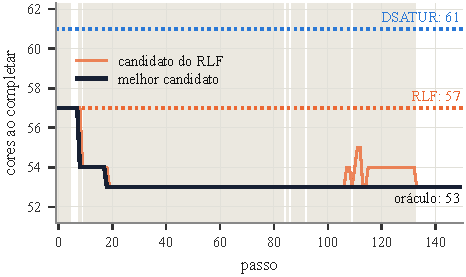
\includegraphics[width=\columnwidth]{rotulo}
\caption{Valor do melhor candidato (oráculo) e do candidato do RLF ao longo da construção no
grafo \texttt{er\_n150\_p0.90\_s0}; as faixas sombreadas são os passos informativos.}
\label{fig:rotulo}
\end{figure}

\subsection{Análise exploratória}
A análise foi implementada como um script que gera um relatório com sete seções, figuras e
tabelas a partir da base, e como um \emph{notebook} interativo que reproduz o mesmo relatório
com células de exploração. As análises cobrem: a visão geral da base; o desempenho das
heurísticas por região do espaço de parâmetros; a informação mútua entre atributos globais e a
heurística vencedora; a escala; as trajetórias por passo; os rótulos por passo; e as
implicações para o modelo.

\subsection{Prova de conceito do modelo}\label{sec:modelo}
\textbf{Formulação.} A cada passo, as quatro heurísticas sugerem candidatos, como no
\emph{rollout}; um classificador binário estima a probabilidade de cada candidato ter rótulo
1; a \emph{política aprendida} colore o de maior probabilidade, com o mesmo desempate do
oráculo. O treino usa apenas os passos \emph{informativos}, aqueles em que ao menos um
candidato tem rótulo 0; nos demais, qualquer escolha dá o mesmo resultado.

\textbf{Atributos (33).} Do candidato: grau, saturação, vizinhos não coloridos e coloridos,
menor cor disponível (\texttt{avail\_color}) e se ela abre cor nova. Do passo: cores já
usadas, fração já colorida e número de candidatos. Relativos: \texttt{avail\_color} e
saturação divididas pelo número de cores já usadas, fração de vizinhos não coloridos e grau
relativo a $n$. Posição entre os candidatos do passo: posto percentual e diferença para o
mínimo de cada atributo do candidato. Quais heurísticas sugeriram o candidato. E um atributo
global por bloco redundante da análise exploratória: $n$, densidade, coeficiente de variação
dos graus e agrupamento relativo à densidade. A mesma função calcula os atributos no treino e
na política, o que um teste verifica.

\textbf{Modelos e divisão.} Comparamos regressão logística com variáveis padronizadas e
\emph{gradient boosting} baseado em histogramas~\cite{friedman2001,ke2017} (300 iterações,
taxa 0,1, até 31 folhas). A divisão treino/validação é \emph{por grafo}, 80/20, estratificada
por família e $n$: 650 grafos e 105.277 passos informativos no treino; 163 grafos e 27.898
passos na validação.

\textbf{Avaliação.} Medimos: (i)~o acerto por passo nos passos informativos de validação,
contra as linhas de base de seguir cada heurística, escolher o candidato de menor cor
disponível e escolher ao acaso; (ii)~o número de cores \emph{de ponta a ponta}, colorindo cada
grafo de validação com a política; (iii)~a generalização para os 551 grafos da réplica 3 da
camada A, que não estão na camada B, incluindo $n>500$; e (iv)~o teste final no DIMACS.

\textbf{Teste final.} O conjunto DIMACS reúne as 79 instâncias de coloração da página original
do desafio~\cite{trickcolor} e 48 instâncias de coloração das séries
COLOR02/03/04~\cite{color04} (Insertions, FullIns, GPIA, mug, quasigrupos, wap e C2000.5 e
C4000.5), num total de 127. O número cromático conhecido vem das próprias páginas, quando
informado (69 instâncias). O modelo, congelado após a prova de conceito, foi aplicado uma única
vez a cada instância; o resultado de cada uma é gravado com o \emph{hash} do modelo e
reexecuções não o sobrescrevem. O oráculo foi calculado como referência nas instâncias com
$n\le500$.

% =====================================================================================
\section{Resultados e discussão}\label{sec:res}

\subsection{Heurísticas na base sintética}\label{sec:res-eda}
A Tabela~\ref{tab:heuristicas} e a Fig.~\ref{fig:vencedora} resumem a camada A. A disputa é
apenas entre RLF e DSATUR: Welsh-Powell e a ordem aleatória nunca são estritamente as
melhores. A família do grafo quase decide a vencedora: o RLF é a única melhor em 89\% dos
grafos ER, e o DSATUR é a melhor (com empate) em todos os BA e a única melhor em 73\% deles; os
empates concentram-se em grafos pequenos ou esparsos, que usam poucas cores. Em média, o RLF
usa 3,1\% de cores acima da melhor heurística; o DSATUR, 5,0\%; o Welsh-Powell, 16,4\%; e a
ordem aleatória, 36,9\%. O padrão se mantém na camada S, com até 10.000 vértices: o RLF supera o
DSATUR em todos os grafos ER e em nenhum BA. O custo é pequeno: em $n=1000$, a mediana do
tempo é de 0,05~s para o DSATUR e 0,09~s para o RLF.

\begin{table}[t]
\centering
\caption{Heurísticas na camada A: fração de grafos em que cada uma é a melhor (com empate) e a
única melhor, e excesso médio de cores sobre a melhor}\label{tab:heuristicas}
\footnotesize
\tabela{heuristicas}
\end{table}

\begin{figure*}[t]
\centering
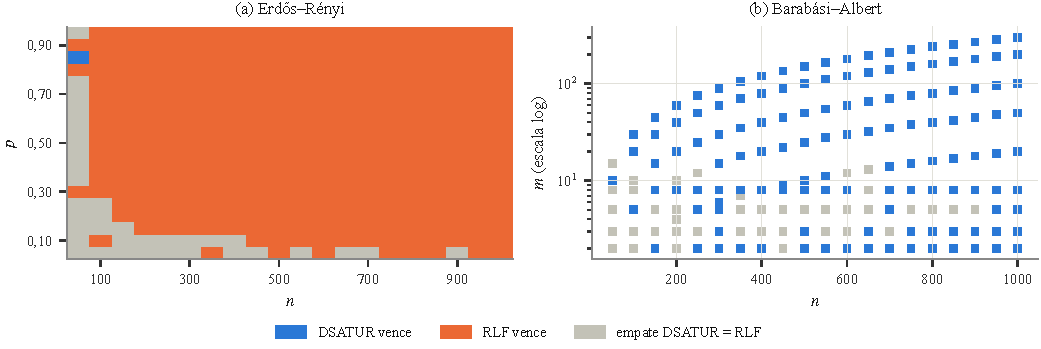
\includegraphics[width=\textwidth]{vencedora}
\caption{Heurística vencedora por região da camada A (moda das 5 réplicas): (a)~grafos ER em
função de $n$ e $p$; (b)~grafos BA em função de $n$ e $m$.}
\label{fig:vencedora}
\end{figure*}

\textbf{Atributos globais.} A informação mútua entre atributos e vencedora, normalizada pela
entropia da vencedora, é maior para o coeficiente de variação dos graus (0,59), o
agrupamento relativo à densidade (0,58) e a razão entre degenerescência e grau máximo (0,58).
Todos separam sobretudo ER de BA; dentro de cada família, os mais informativos são o grau
máximo no ER (0,50) e o grau mínimo no BA (0,19). Há três blocos de atributos quase
redundantes ($|\rho|\ge0{,}95$): \{arestas, grau mínimo, grau médio, degenerescência\},
\{densidade, agrupamento\} e \{coeficiente de variação, grau máximo relativo, degenerescência
relativa\}. Um seletor por grafo tenderia, portanto, a aprender a família geradora.

\textbf{Trajetórias.} As heurísticas constroem a coloração de formas estruturalmente
diferentes (Fig.~\ref{fig:ritmo}): no ER, quando metade dos vértices está colorida, o DSATUR
já abriu 80\% de suas cores e o RLF, 48\%; no BA, o DSATUR abre 97\% das cores nos primeiros
10\% dos passos. Atributos como cores já usadas e menor cor disponível têm, portanto,
distribuições diferentes conforme a regra que gerou o estado: um modelo treinado em estados
de uma política verá outros estados ao seguir a própria.

\begin{figure}[t]
\centering
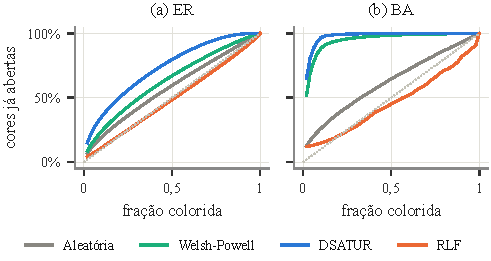
\includegraphics[width=\columnwidth]{ritmo}
\caption{Fração das cores finais de cada heurística já abertas ao longo da construção (média
na camada A).}
\label{fig:ritmo}
\end{figure}

\textbf{Rótulos por passo.} Em 81\% dos passos as quatro sugestões são distintas, mas só
58,6\% dos passos são informativos: 82\% no ER e apenas 6\% no BA, no qual quase todas as
sugestões levam ao mesmo número de cores (Fig.~\ref{fig:passos}a). Nos passos informativos,
o rótulo 1 cobre 42,7\% dos candidatos e o melhor e o pior candidato diferem, em média, por
1,6 cor. A sugestão do RLF é ótima em 88,3\% desses passos, a do DSATUR em 35,1\%, e escolher
ao acaso acerta 42,8\%; perto do fim da construção, a sugestão do DSATUR passa a ser a melhor
(Fig.~\ref{fig:passos}b). Entre as regras de um único atributo, escolher o candidato de menor
cor disponível acerta 81,9\%, o que é essencialmente o princípio do RLF: completar a classe de
cor atual antes de abrir outra. O oráculo supera a melhor heurística em 55\% dos grafos da
camada B (73\% no ER, com ganho médio de 1,5 cor e máximo de 9; 13\% no BA) e nunca fica
pior, como garante a Proposição~\ref{prop:oraculo}.

\begin{figure*}[t]
\centering
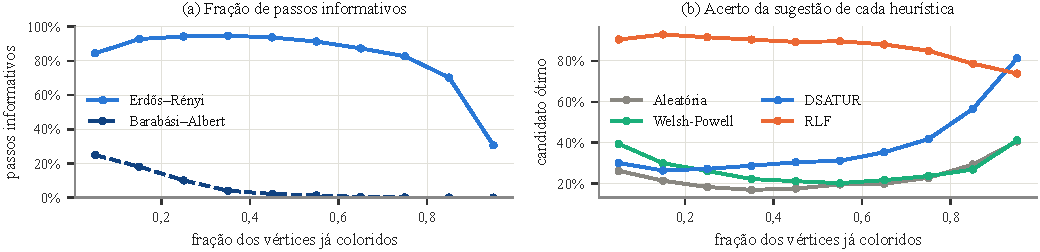
\includegraphics[width=\textwidth]{passos}
\caption{Camada B ao longo da construção: (a)~fração de passos informativos;
(b)~fração dos passos informativos em que a sugestão de cada heurística é ótima.}
\label{fig:passos}
\end{figure*}

\subsection{Prova de conceito}\label{sec:res-modelo}
\textbf{Por passo.} O \emph{gradient boosting} acerta 97,2\% das escolhas nos passos
informativos de validação (98,3\% no treino), contra 93,1\% da regressão logística e 89,3\% da
sugestão do RLF (Tabela~\ref{tab:passo}). A importância por permutação~\cite{breiman2001}
indica que o atributo mais relevante é, de longe, se o RLF sugeriu o candidato (queda de 0,15
na AUC quando embaralhado), seguido da menor cor disponível relativa ao número de cores já
usadas (0,03).

\begin{table}[t]
\centering
\caption{Acerto por passo nos passos informativos de validação}\label{tab:passo}
\footnotesize
\tabela{passo}
\end{table}

\textbf{De ponta a ponta.} A Tabela~\ref{tab:ponta} compara o número de cores da política com
o da melhor das quatro heurísticas em cada grafo. Nos grafos de validação, a política empata
em 96\% dos casos, usa menos cores em 2\% e mais em 2\%; fica, em média, 1,17 cor acima do
oráculo. A regressão logística, com 93\% de acerto por passo, nunca supera a melhor heurística
e perde em 55\% dos grafos BA. Nos 551 grafos da réplica 3, nunca vistos, a política usa menos
cores em 2\% e mais em 7\%; com $n>500$, fora da faixa de tamanhos do treino, menos em 4\% e
mais em 8\% (Fig.~\ref{fig:generalizacao}). A política é mais lenta que as heurísticas, pois
calcula as quatro sugestões e consulta o modelo a cada passo: cerca de 4,7~s por grafo com
$n>500$, contra menos de 0,1~s do RLF.

\begin{table}[t]
\centering
\caption{Política aprendida de ponta a ponta: fração de grafos em que usa menos ($<$), o mesmo
número ($=$) ou mais ($>$) cores que a melhor heurística e diferença média
$\bar{\Delta}$}\label{tab:ponta}
\footnotesize
\tabela{ponta}
\end{table}

\begin{figure}[t]
\centering
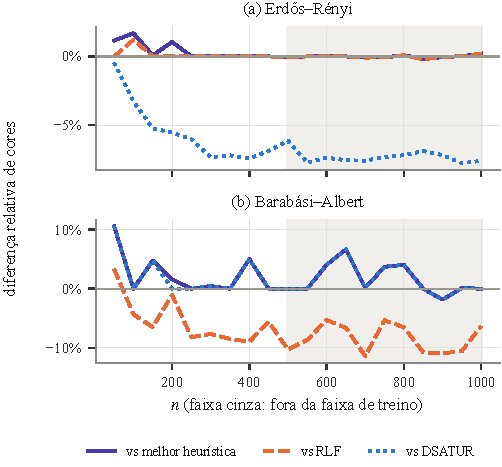
\includegraphics[width=\columnwidth]{generalizacao}
\caption{Diferença relativa de cores da política aprendida em relação à melhor heurística, ao
RLF e ao DSATUR, por $n$, nos grafos da réplica 3 (negativo = política melhor).}
\label{fig:generalizacao}
\end{figure}

\textbf{Por que o acerto por passo não vira menos cores.} Primeiro, a política aprendeu a
\emph{escolher a heurística certa para a família}: ao colorir, seguiu a sugestão do RLF em
98\% dos passos nos grafos ER e a do DSATUR em 93\% nos BA, exatamente as vencedoras da
análise exploratória. Segundo, os erros se acumulam: um grafo de validação tem, em média, 195
passos informativos, e 2,8\% de erro corresponde a cerca de 5 escolhas não ótimas por grafo,
cada uma podendo custar uma cor, enquanto o ganho possível (oráculo) é de pouco mais de uma
cor. Terceiro, os rótulos descrevem os estados do oráculo; após o primeiro desvio, a política
visita estados fora dessa distribuição. A acurácia por passo, sozinha, é uma métrica
enganosa para este problema: o que importa é o número final de cores ao seguir a política.

\subsection{Teste final no DIMACS}\label{sec:res-dimacs}
As 127 instâncias vão de 11 a 10.000 vértices, em 18 famílias, e 69 têm número cromático
conhecido na fonte. Muitas estão fora da região coberta pelo treino (Fig.~\ref{fig:dimacs}a):
há grafos esparsos com graus heterogêneos, como os de atribuição de frequências (wap) e os
GPIA, e grafos estruturados, como Mycielski, Insertions/FullIns e rainhas.

Nas heurísticas, o RLF é o melhor (com empate) em 95\% das instâncias e o único melhor em
38\%; o DSATUR é o melhor em 61\% e o único melhor em 5\%; o Welsh-Powell e a ordem aleatória
nunca são os únicos melhores. Há muitos empates, sobretudo nas famílias estruturadas.

A política aprendida, aplicada sem nenhum ajuste, empata com a melhor heurística em 114
instâncias (90\%), usa menos cores em uma (\texttt{le450\_15c}: 22 cores, contra 23 do RLF) e
mais em 12 (9\%), com diferença média de $+0{,}17$ cor (Tabela~\ref{tab:dimacs}). Ela atinge o
número cromático conhecido em 64\% das 69 instâncias, a mesma fração do RLF
(Tabela~\ref{tab:dimacs-otimo}). As perdas revelam o comportamento de seletor por família:
as instâncias wap são esparsas, têm graus heterogêneos (coeficiente de variação $\approx0{,}5$,
mais próximo dos BA, 0,75, que dos ER, 0,16, de mesma densidade) e agrupamento de 6 a 25 vezes
a densidade, muito acima de ambos; nelas, a política seguiu a sugestão do DSATUR em
praticamente todos os passos, mas o RLF é melhor em três delas, e a política perdeu em quatro
das oito (Fig.~\ref{fig:dimacs}b). Em \texttt{abb313GPIA}, seguiu o
RLF e terminou com 13 cores, mais que o DSATUR (10) e o próprio RLF (11), o que mostra os erros
se acumulando.

O espaço para aprender existe: nas 89 instâncias com $n\le500$, o oráculo usa menos cores que a
melhor heurística em 24\% delas (ganho médio de 0,54 cor e máximo de 10 em
\texttt{school1\_nsh}: 14 cores, contra 24) e atinge o número cromático conhecido em 38 das 58
com $\chi$ conhecido, contra 37 da melhor heurística; a política fica, em média, 0,62 cor acima
do oráculo. O custo da política cresce rápido com $n$: a mediana é de 11~s para
$500<n\le1000$ e de 199~s para $n>2500$, contra 0,1~s e 2,5~s do RLF.

\begin{table}[t]
\centering
\caption{DIMACS: política aprendida comparada a cada referência (fração das instâncias em
que usa menos, o mesmo número ou mais cores; $\bar{\Delta}$ em cores)}\label{tab:dimacs}
\footnotesize
\tabela{dimacs_resumo}
\end{table}

\begin{table}[t]
\centering
\caption{DIMACS: fração das instâncias com $\chi$ conhecido em que cada método o atinge e
excesso médio de cores sobre $\chi$}\label{tab:dimacs-otimo}
\footnotesize
\tabela{dimacs_otimo}
\end{table}

\begin{figure}[t]
\centering
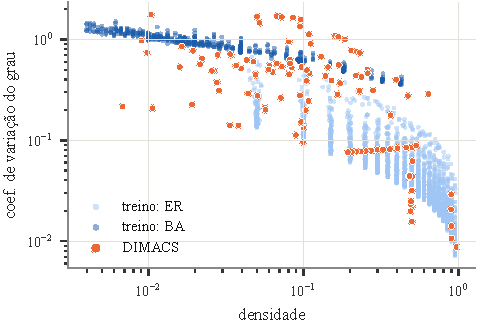
\includegraphics[width=\columnwidth]{dimacs_espaco}\\[2pt]
{\footnotesize (a)}\\[4pt]
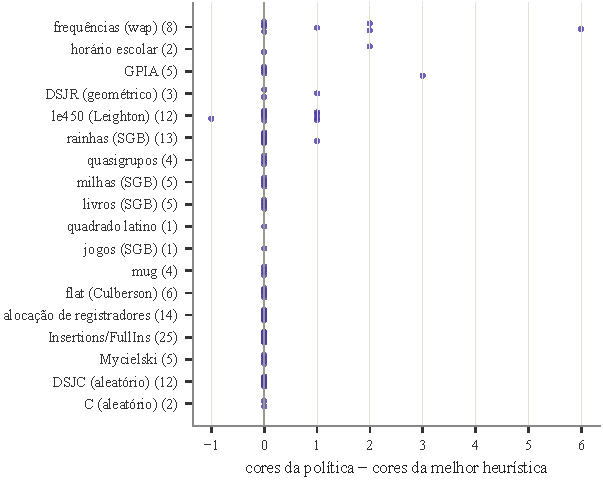
\includegraphics[width=\columnwidth]{dimacs_politica}\\[2pt]
{\footnotesize (b)}
\caption{DIMACS: (a)~instâncias de teste no espaço de atributos do treino (densidade e
coeficiente de variação dos graus, escalas log); (b)~diferença de cores entre a política e a
melhor heurística por instância, agrupada por família (nº de instâncias entre parênteses).}
\label{fig:dimacs}
\end{figure}

\subsection{Limitações e ameaças à validade}
(i)~Os dados de treino são só ER e BA, que ocupam regiões quase disjuntas do espaço de
atributos; outras estruturas, presentes no DIMACS, não estão representadas. (ii)~O modelo só
escolhe entre as sugestões das quatro heurísticas e não pode escolher um vértice que nenhuma
delas indique. (iii)~Os rótulos dependem das políticas-base: um candidato é ``ótimo'' em
relação às conclusões com DSATUR e RLF, não em relação ao ótimo global. (iv)~Usou-se uma única
divisão treino/validação, sem ajuste de hiperparâmetros. (v)~Os números cromáticos conhecidos
vêm das páginas do desafio e podem estar desatualizados em relação à literatura recente.
(vi)~Como o DIMACS foi usado como teste neste trabalho, a avaliação final do POC~II deverá
incluir também um conjunto de teste ainda não utilizado.

% =====================================================================================
\section{Conclusões e trabalhos futuros}\label{sec:conclusao}

O POC~I cumpriu seus objetivos: as quatro heurísticas foram implementadas num arcabouço único
e testado; construiu-se uma base reprodutível de 2.818 grafos sintéticos com rótulos por passo
de qualidade garantida; a análise exploratória mostrou que a disputa é entre RLF e DSATUR,
que a família do grafo quase determina a vencedora e que só parte dos passos exige decisão; e a
prova de conceito mostrou que é possível aprender a escolher entre as sugestões com 97\% de
acerto por passo. O teste final no DIMACS, usado uma única vez, confirmou o quadro observado
nos dados sintéticos: a política empatou com a melhor heurística em 90\% das 127 instâncias e
atingiu o número cromático conhecido na mesma proporção que o RLF (64\%), ao passo que o
oráculo superou a melhor heurística em 24\% das instâncias com até 500 vértices, o que confirma
que há espaço para aprender.

O resultado mais importante é negativo e informativo: acerto alto por passo não basta. A
política aprendida reproduz a melhor heurística de cada família, mas ainda não a supera.

\textbf{As melhorias do modelo ficam para o POC~II.} O plano é:
\begin{enumerate}
\item \emph{Focar nos passos decisivos}: ponderar cada exemplo pela diferença de valor entre os
candidatos ou aprender a ordenar candidatos, para que os erros que custam cores pesem mais.
\item \emph{Treinar onde a política anda}: rotular também os estados visitados pela própria
política, ao estilo do DAgger~\cite{ross2011}, para reduzir a mudança de distribuição.
\item \emph{Otimizar o que importa}: selecionar e ajustar modelos pelo número final de cores de
ponta a ponta e avaliar o ajuste fino por reforço~\cite{khalil2017,watkins2023}.
\item \emph{Ampliar o espaço de escolha e os dados}: considerar candidatos além das quatro
sugestões, possivelmente com GNN~\cite{watkins2023,langedal2024}, e incluir famílias de grafos
estruturados (geométricos, quase $k$-coloríveis, de aplicações) para cobrir a região do
DIMACS.
\item \emph{Reduzir o custo}: calcular as sugestões incrementalmente, como já se faz na
conclusão do RLF, para aproximar o tempo da política ao das heurísticas.
\item \emph{Avaliação mais robusta}: validação cruzada por grafo, ajuste de hiperparâmetros
sem tocar no conjunto de teste e um segundo conjunto de teste ainda não utilizado.
\end{enumerate}

% Sugestão: confira as regras da disciplina sobre declarar o uso de ferramentas de IA. Se for o
% caso, descomente e ajuste:
% \section*{Agradecimentos}
% Partes do código e do texto foram elaboradas com o auxílio de um assistente de IA
% (Claude Code, Anthropic), sob orientação, revisão e responsabilidade do autor.

% =====================================================================================
\bibliographystyle{IEEEtran}
\bibliography{referencias}

% =====================================================================================
\clearpage
\onecolumn
\appendices

\section{Reprodutibilidade}\label{ap:repro}
O código está na pasta \texttt{POC-I} do repositório, com versões fixadas em
\texttt{requirements.txt} (Python 3.13, NumPy 2.4.4, pandas 3.0.2, NetworkX 3.6.1, scikit-learn
1.9.1) e 43 testes automatizados (\texttt{python -m pytest}). A sequência abaixo regenera
todos os resultados deste texto:
\begin{center}
\begin{tabular}{@{}l>{\raggedright\arraybackslash}p{9cm}@{}}
\toprule
Comando & Resultado \\
\midrule
\texttt{scripts/build\_dataset.py} & camadas A, S e B em \texttt{data/} (26 min, 8 processos) \\
\texttt{scripts/eda.py} & relatório da análise exploratória em \texttt{results/eda/} \\
\texttt{scripts/train\_poc.py} & prova de conceito em \texttt{results/poc\_modelo/} (6 min) \\
\texttt{scripts/download\_dimacs.py} & instâncias e catálogo do DIMACS em \texttt{data/dimacs/} \\
\texttt{scripts/process\_dimacs.py} & teste final em \texttt{results/dimacs/} (uso único) \\
\texttt{scripts/paper\_figs.py}, \texttt{paper\_tables.py} & figuras e tabelas deste texto \\
\bottomrule
\end{tabular}
\end{center}

\section{Resultados completos no DIMACS}
\tabela{dimacs_completa}

\end{document}
